\section{Materials and Methods}

\subsection{Datasets}
The main dataset used for validation and comparison is BU3DFE \cite{BU3DFE}. Later BU3DFE is merged with other two multimodal datasets for FER: CalD3r, MenD3s \cite{CalD3rMenD3s} and Bosphorus \cite{Bosphorus} and test the model. \\

\textbf{BU3DFE} \hspace{0.2cm} The Binghamton University 3D Facial Expression Database (BU3DFE) \cite{BU3DFE} is a 3D facial expression database that contains 100 subjects with 2500 samples ($1300\times900$) in two modalities: RGB and 3d mesh. The database includes 7 facial expressions: neutral, anger, disgust, fear, happiness, sadness, and surprise. The dataset is posed because subjects are requested to mimic expressions in 4 intensity levels per emotion (except for neutral which only contain 1 intensity level). The resolution is $512\times512$. 

Following common practice, 3D meshes are converted into depth maps by rendering each mesh in 3D space and extracting the depth value. Getting depth maps that are spatially consistent with corresponding RGB images is challenging because \cite{BU3DFE} gives no information about the camera device used to capture the RGB image (in particular FOV is not defined). Figure \ref{BU3DFE_img} shows an example of reconstruction where we can see the RGB image (a), the corresponding 3D mesh (b) and the depthmap extracted from the mesh (c).\\

\begin{figure}[H]
   \centering
   \begin{subfigure}{0.23\textwidth}
       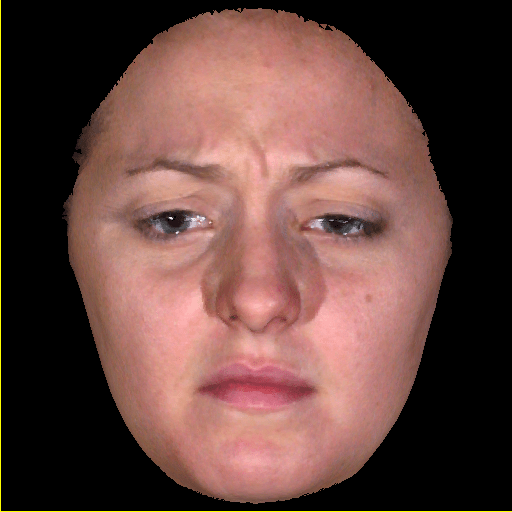
\includegraphics[width=0.8\linewidth]{Images/BU3DFE_rgb.png}
       \caption{}
       \label{BU3DFE_img_a}
   \end{subfigure}
   \begin{subfigure}{0.23\textwidth}
       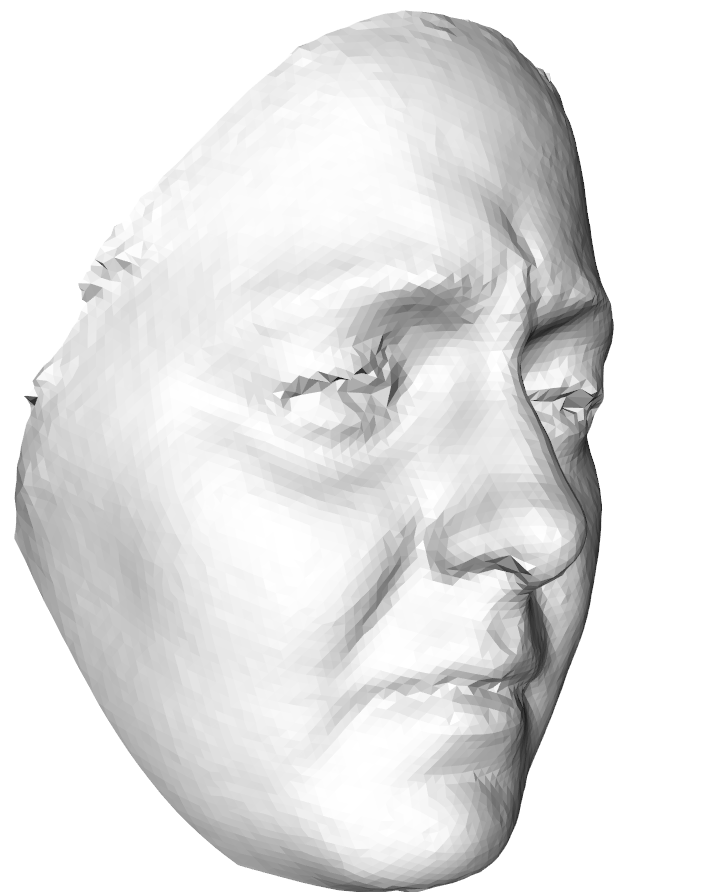
\includegraphics[width=0.8\linewidth]{Images/BU3DFE_mesh.png}
       \caption{}
       \label{BU3DFE_img_b}
   \end{subfigure}
   \begin{subfigure}{0.23\textwidth}
       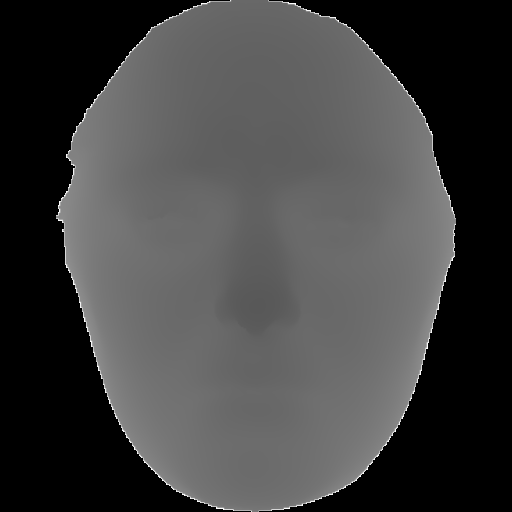
\includegraphics[width=0.8\linewidth]{Images/BU3DFE_depth.png}
       \caption{}
       \label{BU3DFE_img_c}
   \end{subfigure}
   \caption{(a) RGB, (b) 3D Mesh, (c) extracted Depth Map from BU3DFE \protect\cite{BU3DFE}}
   \label{BU3DFE_img}
\end{figure}


 \textbf{CalD3r and MenD3s} \hspace{0.2cm} In CalD3R there are 104 subjects, 54 woman and 50 men mostly from South Europe with age range 19-35 years old. Instead MenD3S comprises 92 subjects, 46 woman and 46 men from Brazil and age range 18-55. The CalD3r and MenD3s dataset \cite{CalD3rMenD3s} are merged into a unique multimodal dataset containing RGB and depth map modalities. The resulting dataset contains 8617 samples annotated with the basic 7 expressions in $224\times224$ resolution. The dataset is spontaneous since expressions are elicited by submitting images to subjects from the International Affective Picture System (IAPS) \cite{IAPS} and the Geneva Affective Picture Database (GAPED) \cite{GAPED}. Slight occlusions can be present on some images, such as those caused by hair, beard, and glasses. Different head poses are naturally portrayed. Each sample is described by RGB and Depth map acquired with Intel RealSense SR300 camera.\\



  \textbf{Bosphorus} \hspace{0.2cm} The Bosphorus dataset \cite{Bosphorus} is a 3D facial expression dataset that contains 105 subjects with a total of 466 samples annotated in 7 classes. Other images are annotated with Action Units. Following the indications provided in CK+ \cite{CK+} the most expressive AUs are translated into categorical annotations. Such translation is provided in Table \ref{AU_translation}. Subjects (60 men and 45 women), with age range 25-35, are mostly Caucasian. The RGB image resolution is $1600\times1200$ and the meshes consist of approximetely $35000$ points each. Finally, this is a posed database as the subjects are requested to mimic the expressions.\\


\begin{table}[H]
    \centering
    \caption{Bosphorus AUs to Categorical conversion}
    \begin{tabular}{cc}
    \hline
    AUs & Class\\
    \hline
    Lip Presser (AU24)  & Anger\\
    \hline
    Nose Wrinkler (AU9) & Disgust\\
    \hline
    Lip Corner Puller (AU12) & Happiness\\
    \hline
    Lip Corner Depressor (AU15) & Sadness\\
    \hline
    Outer Brow Raiser (AU2) & Surprise\\
    \hline
    Inner Brow Raiser (AU1) & Fear\\
    \hline
    \end{tabular}
    \label{AU_translation}
\end{table}


The three datasets distributions are shown in Figure \ref{dataset_distribution}.
\begin{figure}[ht]
\hspace{-0.6cm}
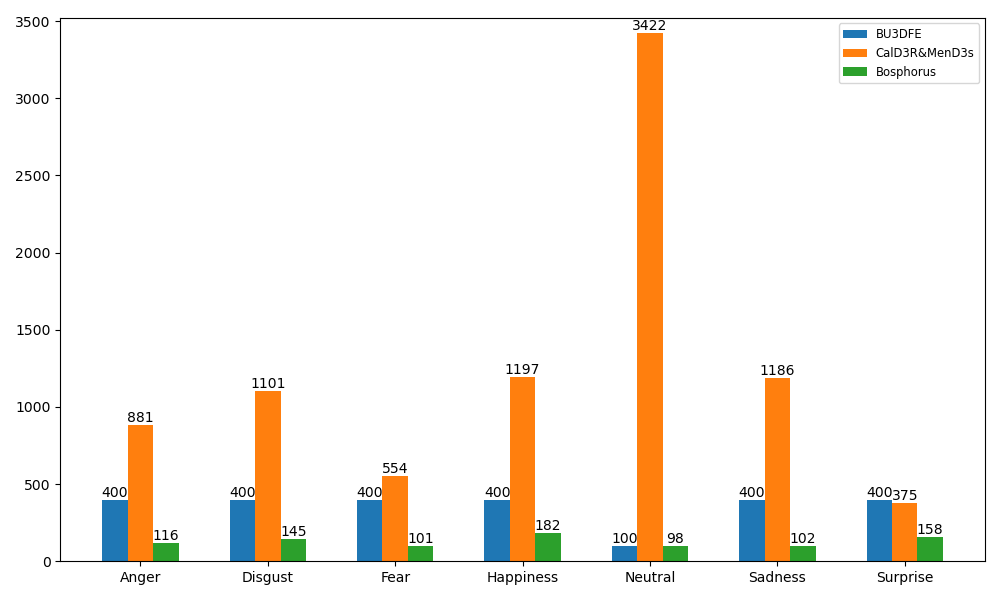
\includegraphics[width=1.2\columnwidth]{Images/Plot0.png}
\caption{Classes distribution of the CalD3rMenD3s, BU3DFE and Bosphorus datasets.}
\label{dataset_distribution}
\end{figure}

\subsection{Preprocessing}

In all datasets, faces have been already cropped to remove background. Depth images, consisting of 1 channel, are stacked to reach default network input used for RGB stream. 
    To leverage EfficientNetB2 pre-trained model from \cite{RW_7_EFF1}, the input images are resized to $260 \times 260$ with linear interpolation.
    Pixels values are rescaled into $[0,1]$ range and z-score normalize as shown in equation \ref{z-score}. Common practice would require to use the mean and standard deviation of the pretraining set (VGGFace2), but that would not guarantee zero centered data for our training set which is very different from VGGFace2, especially for the depth modality. Therefore, at each validation fold, the mean and standard deviation of the training set are computed separately for the two modalities, and used for normalization.

    
\begin{equation}\label{z-score}%with \bm 
    \bm{X_{norm}} = \frac{\bm{X}/max(\bm{X})) - \bm{\mu}}{\bm{\sigma}}
\end{equation}

Data augmentation will help the model to learn robust patterns to variations in lighting, angle, occlusions, etc.. Furthermore, data augmentation could help reducing inter-class similarity as it provides more diverse examples for each class. On the other hand, introducing overly complex data augmentation could introduce unrealistic noise. Online augmentation is chosen as it provides a continuous stream of diverse variations during training process without requiring additional storage. A limited set of realistic augmentations, are selected: 0°-10° rotations, horizontal flips, color jittering (only for RGB images) which simulates variations in lightning and random erasing which simulates occlusion. Data augmentation is not applied on validation samples as they should represent real world conditions to provide an accurate measure of model performance.


\subsection{Network architecture}

Let $I_{rgb}$ and $I_{depth}$ be the RGB and depth images respectively. Resizing and channel stacking for depth images are applied such that $I_{rgb}, I_{depth} \in \mathbb{R}^{H=260 \times W=260 \times C=3}$.

$I_{rgb}$ and $I_{depth}$ are processed in a two stream network in Figure \ref{full_net}, composed of two identical feature extractors (EfficientNetB2) pretrained for face verification on VGGFace2 \cite{RW_7_EFF2}. The architecture of the EfficientNetB2 backbone is shown in Table \ref{EfficientNetb2_arch}, where $Reps$ is the number of repetitions for a block. Note that kernel size $k$ and stride $s$, in \textbf{Inverted Residual Block} (\textbf{IRB}) are referred to the \textit{Depthwise-Conv}, since the \textit{Pointwise-Conv} is always $1\times1$ with stride 1. Features are extracted after the last IRB leading to $X_{rgb}, X_{depth} \in \mathbb{R}^{H=9 \times W=9 \times C=352}$.

Each Inverted residual block (IRB), shown in Figure \ref{inv_res_block} contains a \textbf{Squeeze-Excite} module which permits to select informative channels and suppress less discriminant ones. The same concept can be applied on the spatial information using \textbf{Spatial Attention Mechanisms}. Coordinate Block Attention Module \cite{CBAM} creates the spatial attention map $C \times 1 \times 1$ by concatenationg the MaxPooling and AvgPooling of the feature and then applying convolution and sigmoid activation, as shown in Figure \ref{Spat_att_img}(a). Instead, this work uses the LANet \cite{LANET} approach that uses additional learnable convolution rather than pooling, as shown in Figure \ref{Spat_att_img}(b). Similarly to TransFER \cite{RW_4_TRANSFER}, $S=4$ spatial Attention Modules are selected and their outputs are MaxPooled, but instead of using drop-out of random attention masks, only batchnorm is used, believing it provides similar regularization effect but without hyperparametrs (no dropout probability).

\begin{figure*}[ht]
    \centering
    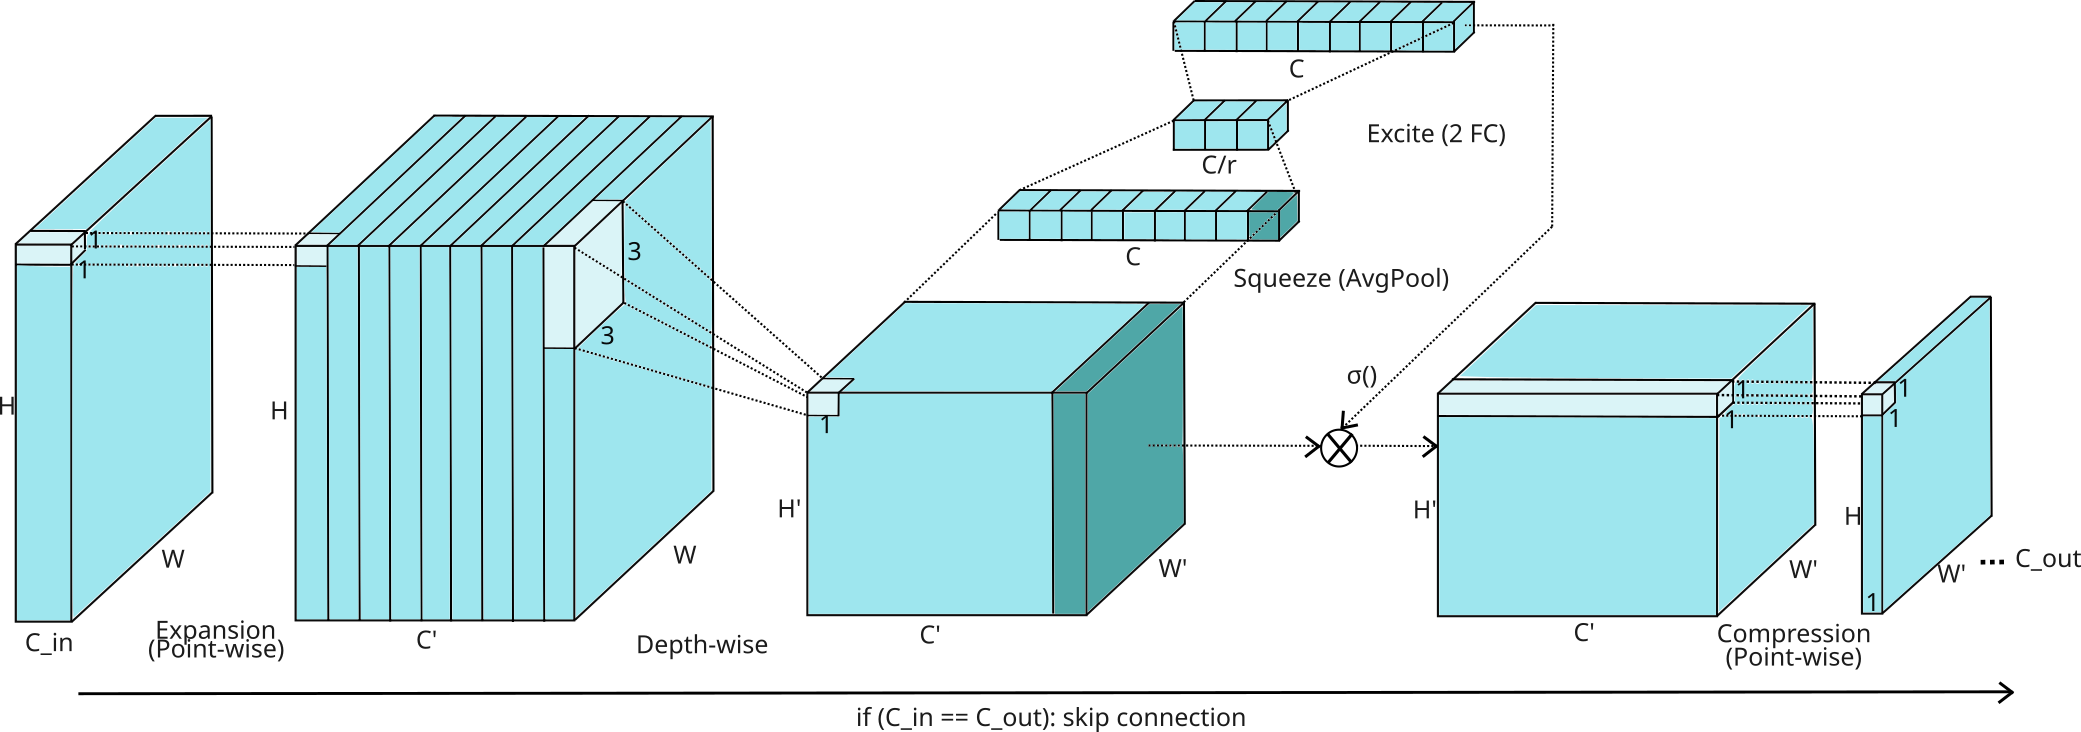
\includegraphics[width=2\columnwidth]{Images/inv_res_block.png}
    \caption{Inverted Residual Block}
    \label{inv_res_block}
\end{figure*}


Moreover, spatial attention is used in a cross modality setup. In particular, the masks $M_{rgb}$ and $M_{depth}$ are computed separately for the two modalities, averaged and multiplied by $X_{rgb}$. The idea is to select the most informative spatial regions from the RGB and Depth stream and average them such that high activations in the RGB image, which could be due to high local illumination, can be suppressed by low activations in the depth image. Viceversa, high activations in the depth image, which could be caused by occlusions, can be suppressed by low activations in the RGB image. In this way the Depth modality is used to guide the learning of the RGB stream.
 
The feature $X_{out}$ is passed through a $1 \times 1$ convolutional layer and reshaped to create a sequence like input for a small Vision Transformer Encoder (only 4 layers). This setup is the same from POSTERV2 \cite{RW_1_POSTERV2}. Finally, two fully connected layers ($MLP$), followed by a softmax layer are used to classify the output.

\begin{figure}[H]
   \centering
   \begin{subfigure}{0.4\textwidth}
       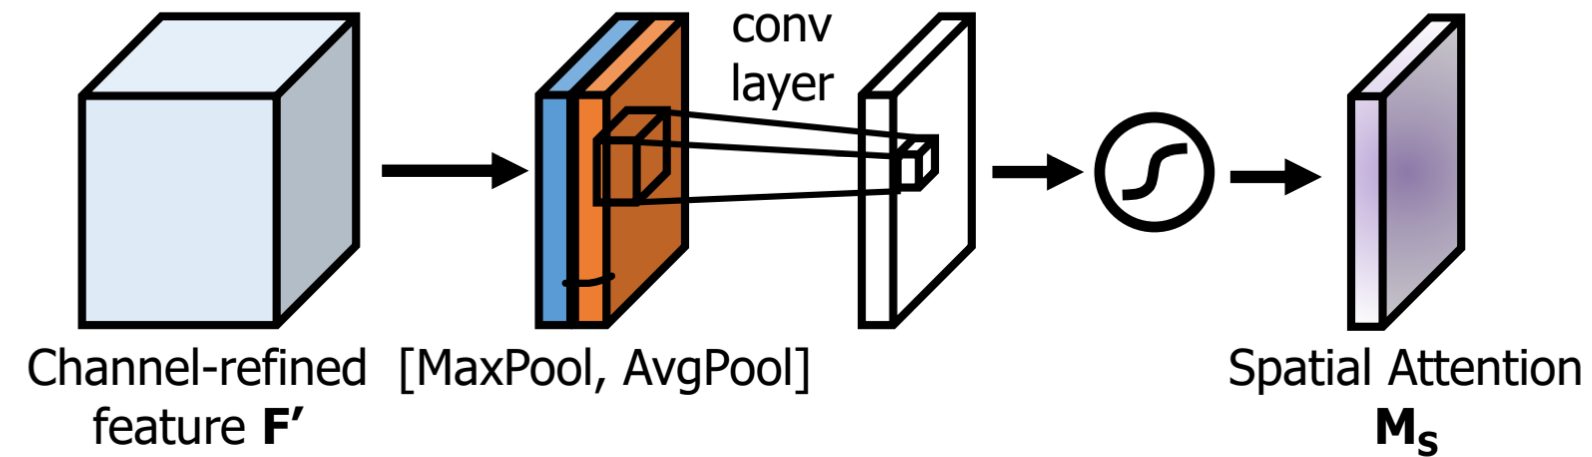
\includegraphics[width=\linewidth]{Images/CBAM.png}
       \caption{}
       \label{Spat_att_img_a}
   \end{subfigure}
   \begin{subfigure}{0.4\textwidth}
       \hspace{0.05cm}
       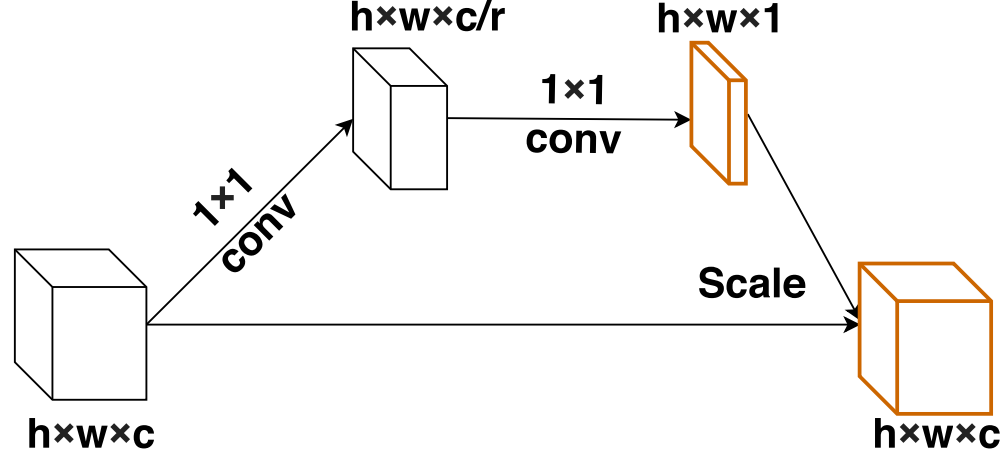
\includegraphics[width=\linewidth]{Images/LANET.png}
       \caption{}
       \label{Spat_att_img_b}
   \end{subfigure}
   \caption{Spatial Attention mechanisms: (a) CBAM \cite{CBAM}, (b) LANet \cite{LANET}}
   \label{Spat_att_img}
\end{figure}


\begin{table}[H]
   \centering
   \caption{EfficientNetB2 Architecture} \label{EfficientNetb2_arch}
   \begin{tabular}{cccccc}
   \hline
   Layer & $C_{in}$ & $C_{out}$ & k & stride & Reps \\
   \hline
   Conv2D (stem) $^a$ & 3 & 32 &$3\times3$& 2 & 1 \\
   \hline
   Conv2D (stem)$^a$ & 32 & 16 & $3\times3$& 2 & 1 \\
   \hline
   IRB $^b$ & 16 & 24 & $3\times3$& 2 & 1 \\
   \hline
   IRB $^b$ & 24 & 24 & $3\times3$& 1 & 2 \\
   \hline
   IRB $^b$ & 24 & 48 & $5\times5$& 2 & 1 \\
   \hline
   IRB $^b$ & 48 & 48 & $5\times5$& 1 & 2 \\
   \hline
   IRB $^b$ & 48 & 88 & $3\times3$& 2 & 1 \\
   \hline
   IRB $^b$ & 88 & 88 & $3\times3$& 1 & 2 \\
   \hline
   IRB $^b$ & 88 & 120 & $5\times5$& 1 & 1 \\
   \hline
   IRB $^b$ & 120 & 120 & $5\times5$& 1 & 3 \\
   \hline
   IRB $^b$ & 120 & 208 & $5\times5$& 2 & 1 \\
   \hline
   IRB $^b$ & 208 & 208 & $5\times5$& 1 & 4 \\
   \hline
   IRB $^b$ & 208 & 352 & $3\times3$& 1 & 2 \\
   \hline
   IRB $^b$ & 352 & 352 & $3\times3$& 1 & 1 \\
   \hline
   Conv2D$^a$ & 352 & 1408 & $1\times1$& 1 & 1 \\
   \hline
   MaxPool & 1408 & 1408 & -& - & 1 \\
   \hline
   FC & 1408 & 7 & -& - & 1 \\
   \hline
   \end{tabular}
   \begin{minipage}{\textwidth}
       \begin{adjustwidth}{0cm}{5cm}
       \caption*{\footnotesize{$^a$ Stem Depthwise Separable block, with batchnorm2D\\
    and SiLU \vspace{0.1cm}\\
       $^b$ Inverted Residual Block. Residual connection is present \\ 
       only if $C_{in}=C_{out}$
       }}
       \end{adjustwidth}
   \end{minipage}
\end{table}

\subsection{Loss Function}

The loss layer is a crucial component of the network, as it defines the objective function that the network aims to minimize during training. The choice of the loss function depends on the specific task and the characteristics of the dataset. In FER context, the loss function should take into account the FER's inherent challenges, in particular the high intra-class variance and high inter-class similarity. Furthermore, FER dataset's are usually very unbalanced as some emotions like surprise or contempt are much more infrequent and/or difficult to annotate with respect to others like anger. \\

In the most  common setting, \textbf{Cross Entropy Loss} reported in Equation \ref{CE loss}, is applied to the output of the softmax layer.
\begin{equation}\label{CE loss}
    \mathcal{L}_{CE} = -\frac{1}{N} \sum^{N}_{i=1}\sum^{K}_{j=1} w_j \thickspace y_{ij} \thickspace  log(p_{ij})
\end{equation}
Where $N$ is the number of samples in the training set. Actually, in deep learning $N$ is the number of samples in the mini-batch. $K$ is the number of classes, $y_{ij}$ is the binary true label for sample $i$ and class $j$ ($y_{ij}=1$ if sample $i$ belongs to class $j$ and $y_{ij}=0$ otherwise).\\
Or in vectorized formulation:
\begin{equation}
    \mathcal{L}_{CE} = -\frac{1}{N} \sum_{i=1}^{N} \bm{w} \cdot \bm{y}_i \cdot \log(\bm{p}_i)^T
\end{equation}
Where $\bm{y}_i$ is the one-hot encoded label vector for $i$th sample.\\

One problem with standard CE loss is that it treats every sample equally, which can be problematic in FER where class imbalance is very common. This can lead to biased models that perform poorly on minority classes. To address this, a weighted version of CE loss can be used, where each class is assigned a weight $w_j$ based on its frequency. This encourages the model to focus more on underrepresented classes, leading to improved performance on imbalanced datasets.\\

To address high intra-class variability and high inter-class similarity problems, center loss permits the network to produce features that are both separable (featuers from different classes are far apart in the feature space) and discriminant (features from same class are close to each other in the feature space and so encoding the class characteristics). The center loss is reported in Equation \ref{eq_center_loss}.\\
\begin{equation} \label{eq_center_loss}
    \mathcal{\bm{L}}_c = \frac{1}{2} \sum_{i=1}^{N} \norm{\bm{x}_i - \bm{c}_{y_{i}}}_{2}
\end{equation}
Where $\bm{c}_{y_{i}}$ is the class center of the class $y_i$. Center loss increases the discriminative power of the features by explicitly penalizing the distance between the deep features $\bm{x}_i$ of each face image and their corresponding class centers in the feature space $\bm{c}_{y_{i}}$. Ideally, the class centers should be learnt by computing the mean of the deep features produced at each step for all the samples of the same class in the training set. However, this would be inefficient and impractical. So, class centers are actually updated at each iteration by averaging the deep features of the samples in the mini-batch \cite{center_loss}. This may introduce large perturbations in the learning of the centers (for example, a mini-batch could contain only samples from a single class with a mean very different from the global mean). To avoid this, the learning rate of the centers is controlled by an hyperparameter $\alpha \in [0,1] $.\\

The limit of center loss is that it only compresses the clusters individually, but does not push clusters apart. This is why it is used in conjunction with CE loss which forces the fetures of different classes to stay apart.\\

In 2017, Cai et al. \cite{island_loss} further developed the center loss to produce even more discriminative features and trained a CNN with Island Loss for FER. The combined loss will be therefore the sum of \textbf{Island Loss}, center loss and CE loss as presented in Equation \ref{isl_combinedloss}.\\

\begin{equation} \label{isl_combinedloss} 
    \mathcal{\bm{L}} = \mathcal{\bm{L}}_{CE} + \lambda_1 \mathcal{\bm{L}}_C + \lambda_2 \mathcal{\bm{L}}_I
\end{equation}  

Where $\lambda_1$ and $\lambda_2$ are hyperparameters that balance the three loss functions. $\mathcal{\bm{L}}_I$ is the Island Loss, defined in Equation \ref{island_loss_eq}.\\

\begin{equation} \label{island_loss_eq} 
        \mathcal{\bm{L}}_I = \sum_{\bm{c}_j}^{K} \sum_{\bm{c}_k \neq \bm{c}_j}^{K} \left(\frac{\bm{c}_j \cdot \bm{c}_k}{\norm{\bm{c}_k}_{2} - \norm{\bm{c}_k}_{2}} + 1\right)
\end{equation}  

$\bm{c}_j$ and $\bm{c}_k$ are the class centers of class $j$ and $k$ respectively. Intuitively, it minimizes the cosine similarity between the class centers, which encourages the features of different classes to be more separable in the feature space. The +1 term is necessary to make the loss non-negative, since the cosine exists in $[-1,+1]$ range.\\
Figure \ref{center_loss_fig} shows the features learned by a CNN trained with Cross Entropy loss (a), Center loss (b) and Island loss (c). Note how the center loss aggregates the features of the same expression class towards their centers, thus reducing intra-class variation with respect to the CE loss (a).\\
The island loss (c) not only compresses the clusters individually but also pushes clusters apart \cite{island_loss}.\\

\begin{figure}[h]
    \centering
    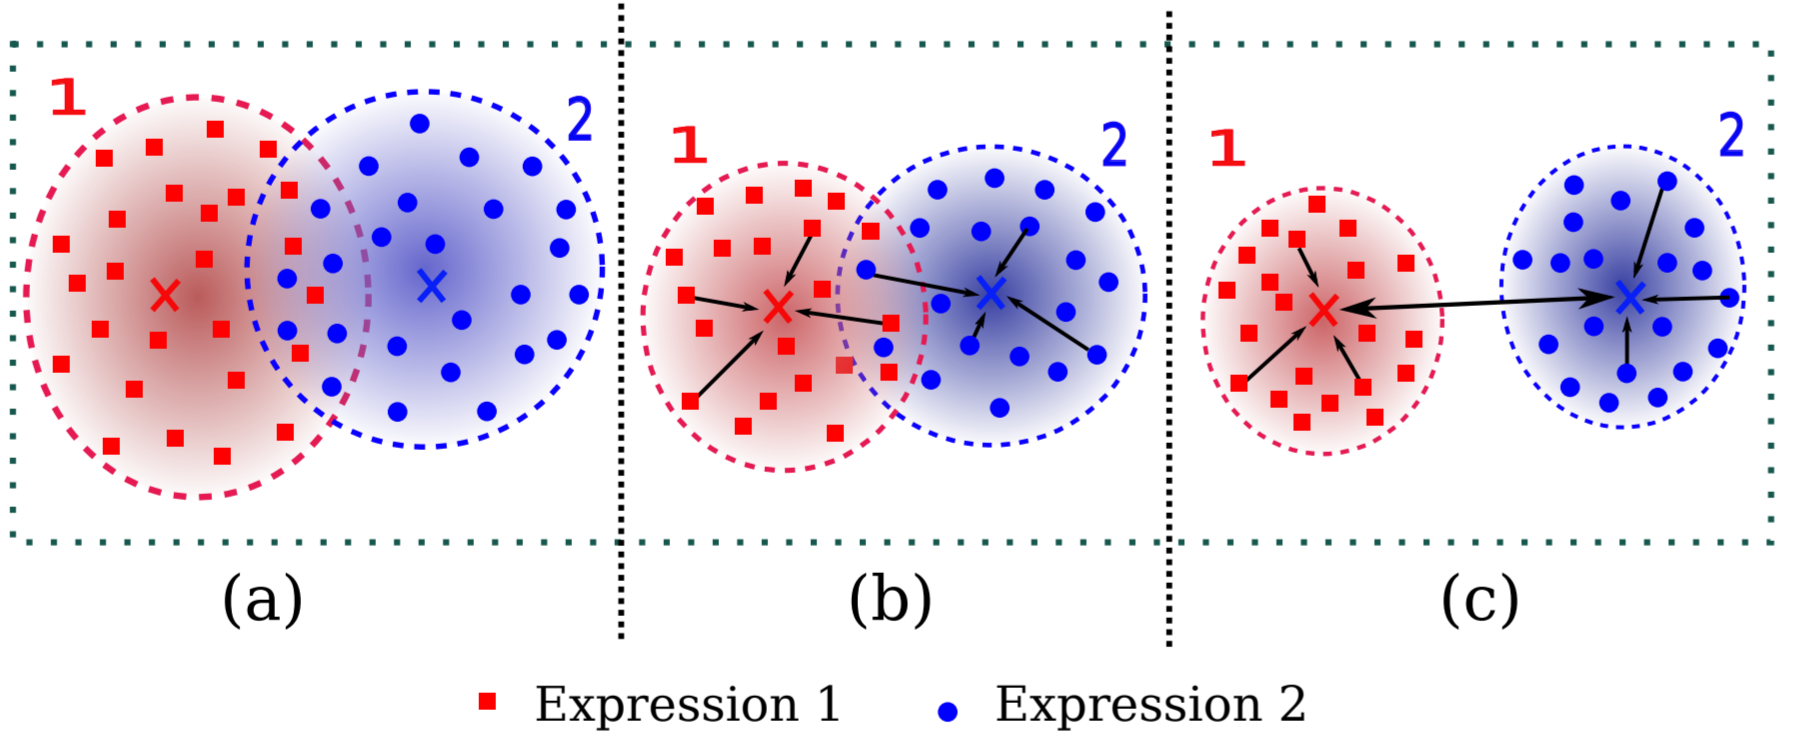
\includegraphics[width=0.85\columnwidth]{Images/center_loss.png}
    \caption{Features learned by a CNN trained with CE loss (a),  Center loss (b), Island loss (c) \protect\cite{island_loss}}
    \label{center_loss_fig}
\end{figure}

Note that other loss functions have been proposed to enhance the discriminative power of the deeply learned features, such as contrastive loss \cite{contrastive_loss}, triplet loss \cite{triplet_loss} which construct the loss function for image pairs and triplets respectively\cite{center_loss}. However, the number of possible pairs and triplets grows quadratically and cubically respectively with the number of samples in the minibatches. A common strategy is to select meaningful pairs and triplets (those that give significant contribute to the training), but these searching algorithm increase training time. In contrast, center loss is computationally efficient and easy to implement, making it a popular choice for enhancing the discriminative power of the features in FER tasks. This comes at the cost of fine-tuning the hyperparameters $\lambda$ to balance the two loss functions, and $\alpha$ to control the learning rate of the centers.

\subsection{Experimental Settings}
Because pretrained backbones are used, the initial weights are biased towards a very different dataset from ours, especially for depth modality. For this reason, common practice suggests to adopt a "warm-up" strategy where the learning rate is initially set to a very low value and then increased to the desired value. This allows the model to slowly adapt to the new dataset without abrupt oscillations caused by large gradients.

A popular learning rate schedule that adopts this strategy is the One-Cycle schedule \cite{superconvergence} where the learning rate starts very low, increases up to a maximum value and then decreases following a cosine annealing schedule. Table \ref{lr_setup} shows the learning rate setup for the two backbones and the "fusion network" (comprising the Cross Modality Spatial Attention, the transformer encoder and the MLP) all using One-Cycle schedule. Note that the maximum value is higher for the fusion network because it is trained from scratch, while the backbones are pretrained and only need to be fine-tuned. The learning rate schedule for the fusion network is shown in Figure \ref{lr_sched}.


\begin{table}[H]
    \centering
    \caption{Learning rate setup}
    \begin{tabular}{cccc}
    \hline
     & Max LR & Min LR & Schedule \\
    \hline
    Backbones & $1^{-4}$ & $10^{-6}$ & One-cycle \\
    \hline
    Fusion Network & $1^{-3}$ & $10^{-6}$ & One-cycle\\
    \hline
    \end{tabular}
    \label{lr_setup}
\end{table}


\begin{figure}[H]
    \centering
    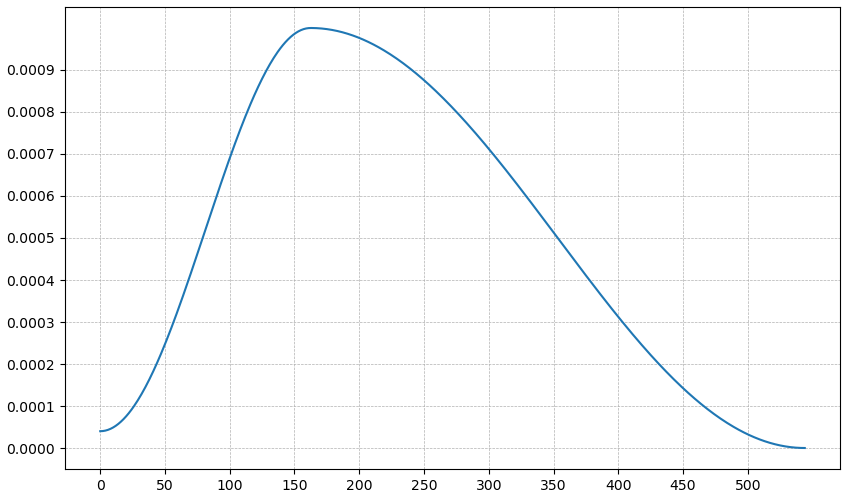
\includegraphics[width=0.8\columnwidth]{Images/onecycle_lr.png}
    \caption{Onecycle learning rate schedule for the fusion network}
    \label{lr_sched}
\end{figure}


\begin{figure*}[ht]
    \centering
    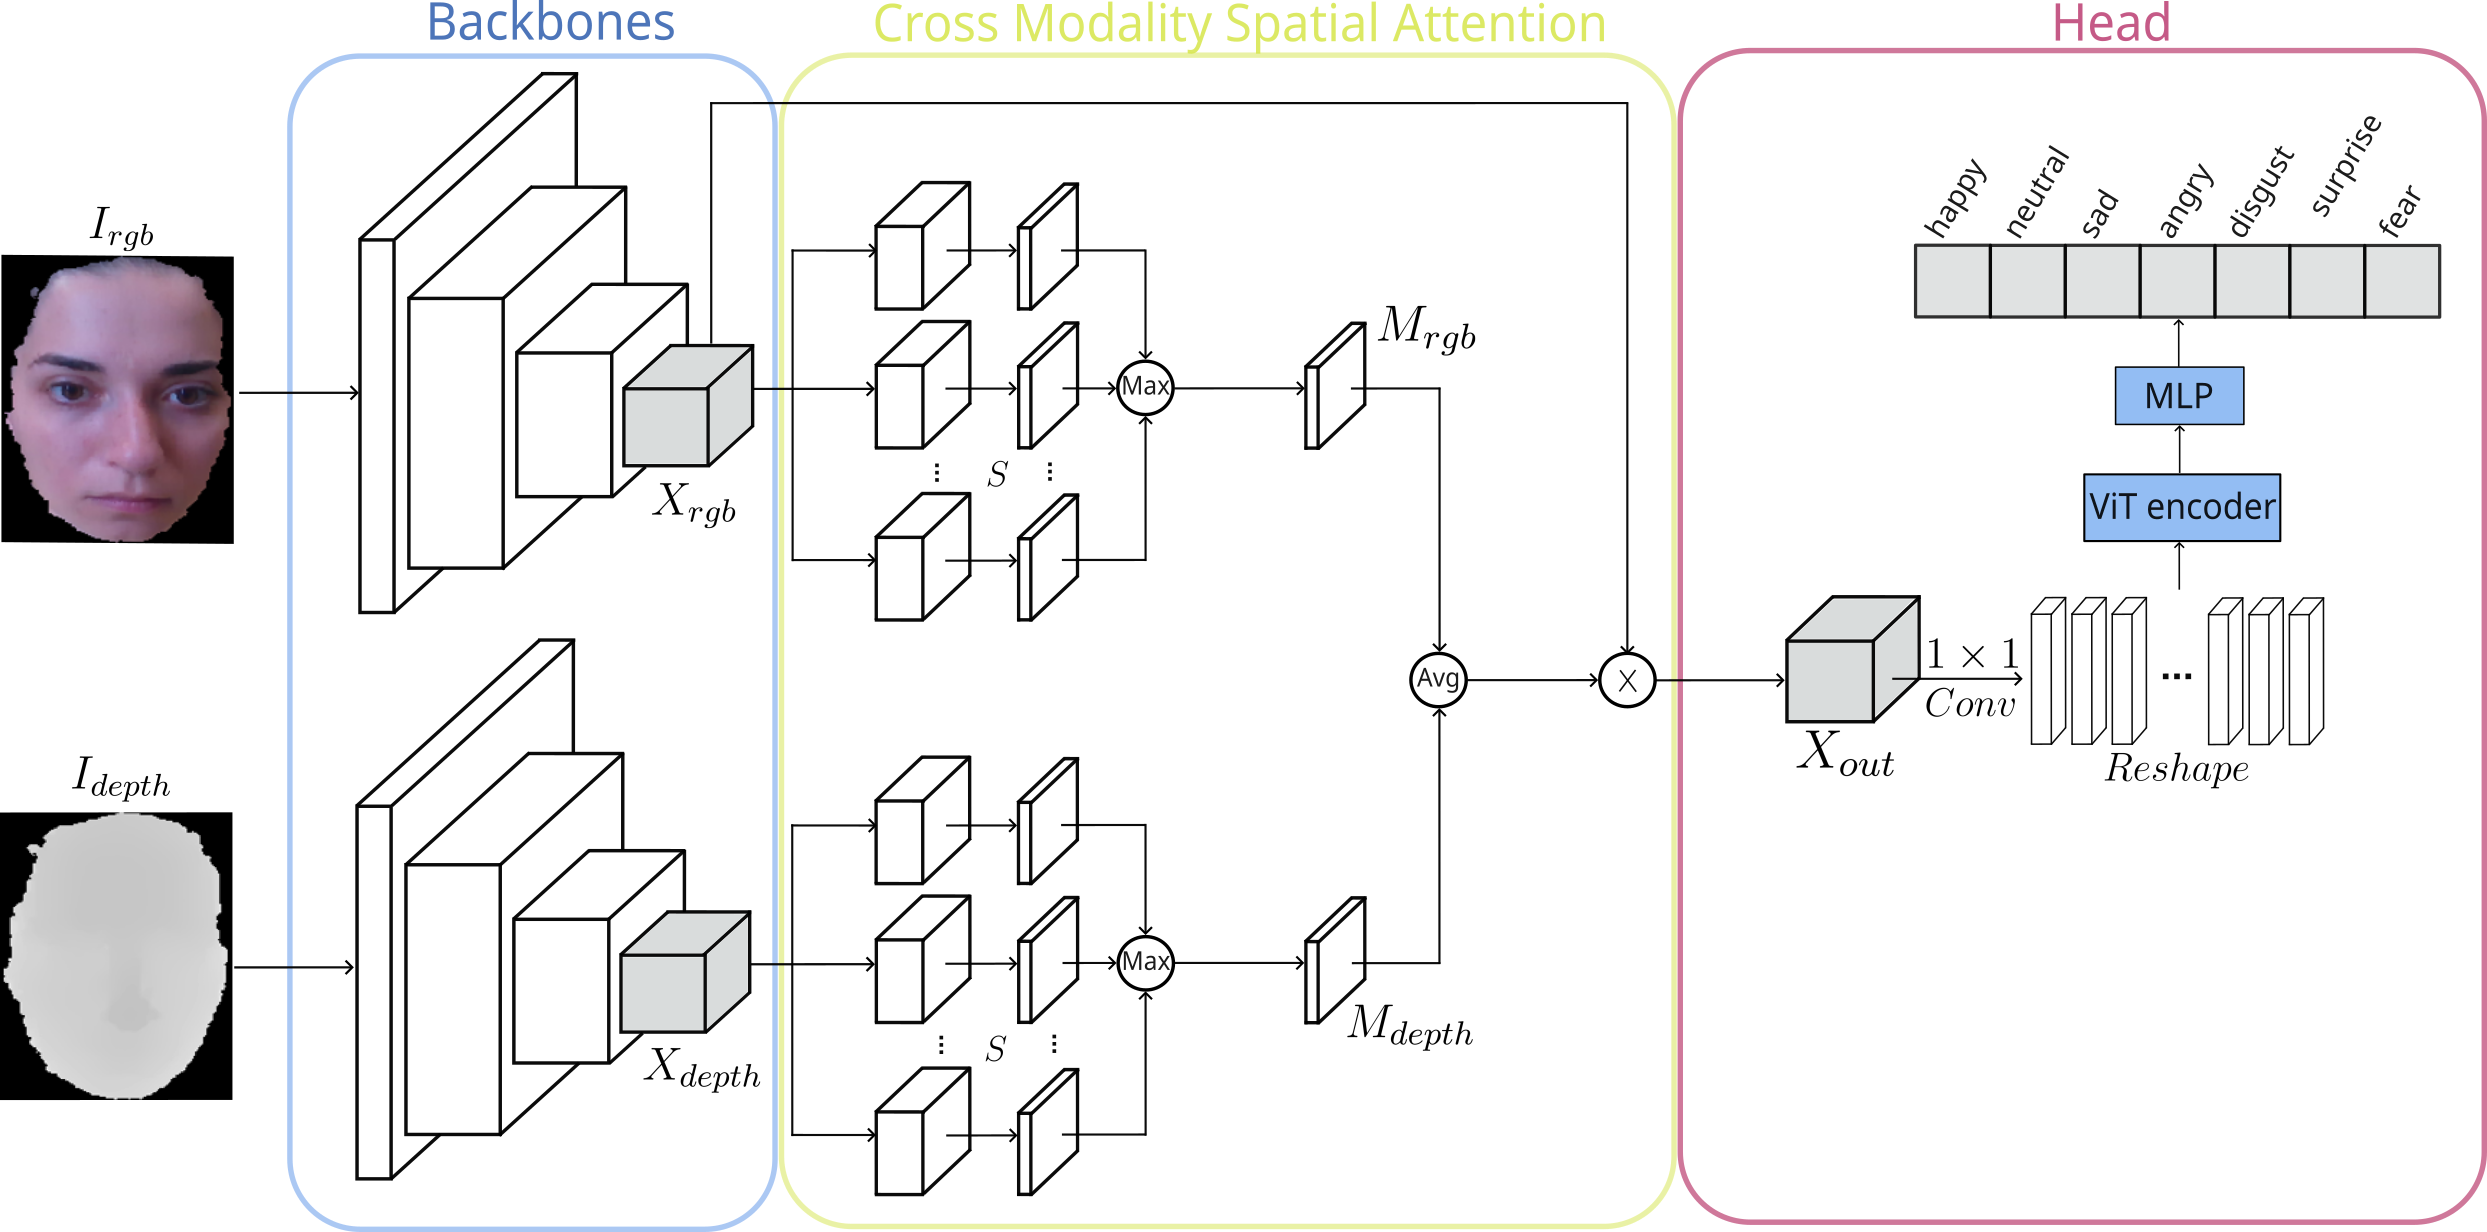
\includegraphics[width=2.2\columnwidth]{Images/full_net.png}
    \caption{Model architecture}
    \label{full_net}
\end{figure*}


AdamW optimizer is used. Island Loss is set up with $\lambda_1=1^{-2}$ and $\lambda_2=10$, with centers learnt using an SGD optimizer with fixed learning rate $\alpha=0.5$.

To make the network faster, Automatic Mixed Precision (AMP) is used to make the forward pass in half precision (16bits) while keeping the weights in single precision (32bits). This allows to reduce the memory usage and the computational time.

Batch size is set to 128 with gradient accumulation to make up for memory constraints. Using relatively small batches allows to introduce a regularization effect in the training due to the noise in the gradients computed on smaller batches with respect to larger ones used in other works (e.g. 1024 in \cite{RW_4B_CLIP} or bigger). These values of batch size, learning rate, weight decay, lambdas and $S$ are hyperparameters tuned through a random search strategy (with Optuna framework \cite{Optuna}) to find the best combination of hyperparameters.

The same strategy from AFNET \cite{RW_8A_AFNET}, CMANET \cite{RW_8B_CMANET}, FFNET \cite{RW_8C_FFNET}, MFEVIT \cite{RW_8D_MFEVIT}, CMFN \cite{RW_9_CMFN}, OGFNET \cite{RW_10_OGFNET} (and others) is used to validate the model over BU3DFE. The neutral class, which is under represented, is discarded and only the 2 highest intensity level images are used. Moreover, only 60 random subjects out of 100 are selected. Finally, 10 fold cross validation is conducted over these 60 subjects, for 100 repetitions, selecting different folds at each repetition. The folds accuracies, inside each repetition, are averaged to get repetition accuracy. Later also the 100 repetition accuracies are averaged to get the final results. \\
This evaluation protocol is difficult to reproduce because the 60 subjects are selected once at the beginning and it may happen that "easy" subjects are selected. In fact, in order to reproduce the same experiment, the 60 subjects should be the always the same, but the above cited works don't share this information. Moreover, the total amount of images used for validation is only $720$ which is very small considering the initial 2500 samples.\\

Therefore, this work sets a new benchmark for BU3DFE, selecting a 5-fold cross validation over the whole dataset (considering all emotional intensity levels and also the neutral class). Therefore, in this second setup the dataset is larger (2500 samples) and larger batch size (256) can be used. Training is performed for approximately 13 epochs.
In every setup, the model is trained for 20 epochs on each fold. Tesla T4 GPU with 12GB memory is used. 


